\documentclass[10pt]{beamer}
\usepackage{fancyvrb}
\usepackage{times}
\usepackage{pgf,pgfarrows,pgfnodes,pgfautomata,pgfheaps}
\usepackage{amsmath,amssymb}
\usepackage[utf8]{inputenc}
\usepackage{colortbl}
\usepackage[portuges]{babel}
\usepackage{graphicx}
\usepackage{color}
\usepackage{hyperref}
\usepackage{pxfonts,txfonts}
\usepackage{url}
\usepackage{underscore}
\usepackage[T1]{fontenc}

\usefonttheme{structurebold}
%insert for WSCAD19
\usepackage{multirow}
\usepackage{subfigure}
\usepackage{multicol}

%==================================================================================
\definecolor{DarkGreen}{rgb}{0,.5,0}
\definecolor{DarkRed}{rgb}{.5,0,0}
\definecolor{DarkBlue}{rgb}{0,0,.5}

\newcommand{\x}{\textbf{\textcolor{DarkGreen}{$\surd$}}}
\newcommand{\xx}{\textbf{\textcolor{DarkBlue}{$\odot$}}}
\newcommand{\xxx}{\textbf{\textcolor{DarkRed}{$\times$}}}
%==================================================================================

\usepackage{listings}
\renewcommand{\lstlistingname}{Programa}

\lstset{
numbers=left,
stepnumber=1,
firstnumber=1,
numberstyle=\tiny,
extendedchars=true,
breaklines=true,
frame=tb,
basicstyle=\footnotesize,
stringstyle=\ttfamily,
showstringspaces=false
}

%==================================================================================

\usetheme{Amsterdam}

%==================================================================================

\usecolortheme{default}
\setbeamertemplate{navigation symbols}{}

% inserir logotipo na apresentação
\pgfdeclareimage[height=0.5cm]{logo}{img/lups_oficial.png}
\logo{\pgfuseimage{logo}}
%Tinha a logo de outros orgãos 
\setbeameroption{hide notes}
%==================================================================================

\title[]{Estudo de viabilidade do uso de Raspberry PI na névoa}
\author[]{\textbf{\underline{Guilherme de Souza}\\ Nelson Lago \\ Prof. Dr. Gerson Cavalheiro\\ Prof. Dr. Alfredo Goldman\\}
Centro de Desenvolvimento Tecnológico\\
%Bolsista PROBIC/PROBITI\\
 WSCAD 2019\\
 gdsdsilva@inf.ufpel.edu.br\\
}

\date{Outubro -- 2019  -- Campo Grande/MS}

%==================================================================================

\begin{document}
\frame[label=titlepage]{\titlepage \vspace{-1cm} \hspace{-1cm}}


\section{Introdução}
\frame{
    \frametitle{Introdução}
    \begin{block}{\textbf{Introdução}}
    \begin{itemize}
      \item 1,4\% da energia mundial é consumida por \textit{datacenters} cujas máquinas possuem uma composição de \textit{hardwares} convencionais com alto consumo energético;
      \item Existem, porém, dispositivos de arquitetura ARM cuja característica principal é o baixo consumo de energia;
      \item Tais dispositivos também são capazes de atender a demanda de uma nuvem. 
    \end{itemize}
  \end{block}
}

%% ---
\frame{
    \frametitle{Nuvem Computacional}
    \begin{figure}[!tbp]
      \centering
      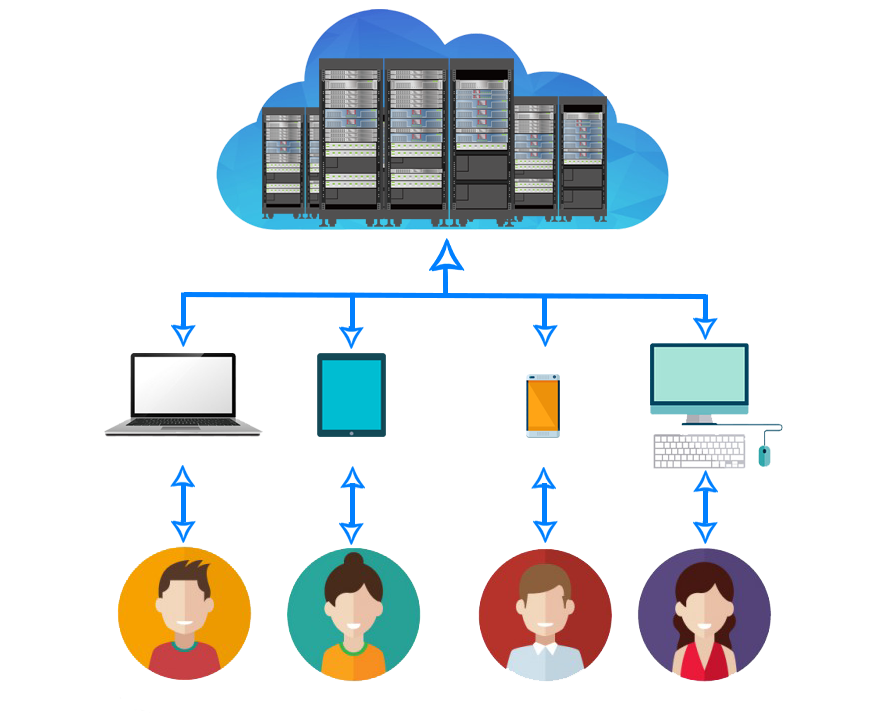
\includegraphics[width=0.80\textwidth]{img/CloudImage.png}\label{fig:f1}
    \end{figure}
}
%% ---

\frame{
  \frametitle{Introdução}
  \begin{block}{Questionamento Central}
    \begin{figure}[!tbp]
      \centering
      
\includegraphics[width=0.25\textwidth]{img/nuvem.png}\label{fig:f1}
    \end{figure}
    \centering{\normalsize \bf \textit{Hardwares} de baixo consumo energético como parte de uma nuvem computacional são viáveis?}
  \end{block}
}
\frame{
  \frametitle{Objetivos}
  \begin{block}{Gerais}
    \begin{itemize}
      \item Comparar a capacidade computacional de dois \textit{hardwares} de baixo consumo utilizando um \textit{benchmark}.  
    \end{itemize}
  \end{block}
  \begin{block}{Específicos}
    \begin{itemize}
      \item Definir o \textit{benchmark} que melhor atende aos objetivos do trabalho; 
      \item Decidir qual \textit{hardware} é o adequado para ser implementado em uma nuvem real.
    \end{itemize}
  \end{block}
}
%% ---

%==================================================================================
\section{Metodologia}
\frame{
  \frametitle{Metodologia}
  \begin{block}{\textit{Especificações}}
    \begin{table}[!h]
      \centering
%      \caption{Especificações do \textit{hardware} dos dispositivos segundo o fabricante. A corrente e a tenão de cada dispositivo corresponde ao valor máximo suportado.}
      \label{tab:espesificacao}
      \begin{tabular}{|c|c|c|} \hline
        \textbf{Especificação} & \textbf{Raspberry PI B+} & \textbf{Raspberry PI 3} \\ \hline
        Processador & \begin{tabular}[c]{@{}c@{}}BCM2835 \\ SINGLE Core 700MHz\end{tabular} & \begin{tabular}[c]{@{}c@{}}BCM2837 64Bit \\ QUAD Core 1.2GHz\end{tabular} \\ \hline
        Arquitetura & ARMv6 & ARMv8 \\ \hline
        RAM & 512MB SDRAM 400MHz & 1GB SDRAM 400MHz \\ \hline
        Amazenamento & Micro SD & MicroSD \\ \hline
        Corrente/Tensão & 0,7A / 5V & 1,34A / 5V \\ \hline
      \end{tabular}
    \end{table}
  \end{block}
}

\frame{
    \frametitle{Metodologia}
    \begin{block}{Benchmark}
        \begin{itemize}
          \item O \textit{benchmark} escolhido foi o \textit{Yahoo! Cloud Serving Benchmark}~(\textbf{YCSB}):
          \begin{itemize}
            \item Mede o desempenho de uma aplicação de banco de dados no dispositivo escolhido;
            \item Obtem informações como vazão de operações e atraso de processamento das requisições.
          \end{itemize}
        \end{itemize}
    \end{block}
}

\frame{
    \frametitle{Metodologia}
    \begin{block}{Execução}
        \begin{itemize}
          \item O teste é divido em duas partes:
          \begin{itemize}
            \item \textit{Load};
            \item \textit{Run}.   
          \end{itemize}
          \item Contém seis testes diferentes:
          \begin{itemize}
            \item \textit{Workload} A à \textit{Workload} F. 
          \end{itemize}
        \end{itemize}
    \end{block}
}

\frame{
    \frametitle{Metodologia}
    \scriptsize
    \begin{block}{Características dos Workloads}
      \begin{table}[!h]
      \centering
      \caption{Características dos \textit{workloads} selecionados para testes.}
      \label{tab:workload}
      \begin{tabular}{|c|c|c|c|c|}
      \hline
      \textit{Workload} & Número de Ops & Leitura & \textit{Update} & Detalhes        \\ \hline
      a        & 1000        & 50\%    & 50\%        & Simula salvar uma sessão        \\ \hline
      b        & 1000        & 95\%    & 5\%        & Simula adição de \textit{tags} a foto      \\ \hline
      c        & 1000        & 100\%   & 0\%        & Simula \textit{cache} de perfil do usuário \\ \hline
      d        & 1000        & 95\%    & 0\%        & 5\% de inserção não ordenadas     \\ \hline
      \end{tabular}
      \end{table}
    \end{block}
}

\frame{
  \frametitle{Metodologia}
  \begin{block}{Metodologia do teste}
    \begin{itemize}
    \item Seguindo a documentação e utilizando um script de execução, que realizava os seguintes passos para cada \textit{workload}:
      \begin{itemize}
        \item Executa o carregamento de chaves através do comando ycsb \textit{load};
        \item Realiza o teste utilizando o comando ycsb \textit{run}, redirecionando a saída para um arquivo txt;
        \item Limpa as chaves do banco de dados. 
      \end{itemize}
    \end{itemize}
  \end{block}
}

\frame{
  \frametitle{Metodologia}
  \begin{block}{Fórmulas}
    \begin{itemize}
    \item Realizou-se o cálculo da potência média e operações por Watt:
      \begin{itemize}
        \normalsize
        \item \textit{Potência = Tensão * Corrente}; 
        \item \textit{Operação por Watt = Média de vazão / Potência}.
      \end{itemize} 
    \end{itemize}
  \end{block}
}

%==================================================================
\section{Resultados}
\frame{
    \frametitle{Resultados}
    \begin{block}{ }
        \begin{table}[!hb]
            \centering
            \caption{Total de escritas e leituras alcançadas com sucesso e falhas ao final de 25 minutos. \label{tab:result_in_table}}
            \begin{tabular}{c|c|c|cc}
                \multirow{2}{*}{\textbf{Experimentos}} & \multicolumn{2}{c|}{\textbf{Escrita}} & \multicolumn{2}{c}{\textbf{Leitura}}                   \\ \cline{2-5} 
                & \textbf{Sucesso}   & \textbf{Falha}   & \multicolumn{1}{c|}{\textbf{Sucesso}} & \textbf{Falha} \\ \hline
                Experimento 1                         & 1.990.963          & 2.585            & \multicolumn{1}{c|}{-}                & -              \\ \hline
                Experimento 2                         & -                  & -                & \multicolumn{1}{c|}{2.155.112}        & 0              \\ \hline
                Experimento 3                         & 834.606            & 26               & \multicolumn{1}{c|}{808.983}          & 0              \\ \hline
            \end{tabular}
        \end{table}
    \end{block}
}

\frame{
    \frametitle{Resultados de escrita}
    \begin{figure}[!ht]
        \centering
        \mbox{%
            \subfigure[Latência de escritas]{\label{avr-prgmem}%
            
\includegraphics[width=0.2\textwidth]{/home/souza/Documents/LUPS/CIC/presentation/img/logoRaspberry.png}}\qquad
            \subfigure[Requisições por segundo]{\label{avr-datamem}%
            
\includegraphics[width=0.2\textwidth]{/home/souza/Documents/LUPS/CIC/presentation/img/logoRaspberry.png}}
            }
            \caption{Latências e requisições por segundo durante escrita no período de execução de 25 minutos desconsiderando os 5 primeiros do simulador.}
            \label{fig:avr-memmap}
    \end{figure}
}

\frame{
    \frametitle{Resultados de leitura}
    \begin{figure}[!hb]
        \centering
        \mbox{%
            \subfigure[Latências de leituras]{\label{avr-prgmem2}%
            
\includegraphics[width=0.2\textwidth]{/home/souza/Documents/LUPS/CIC/presentation/img/logoRaspberry.png}}\qquad
            \subfigure[Operações por segundo]{\label{avr-datamem2}%
            
\includegraphics[width=0.2\textwidth]{/home/souza/Documents/LUPS/CIC/presentation/img/logoRaspberry.png}}
            }
            \caption{Latências e requisições por segundo durante leitura no período de execução de 25 minutos desconsiderando os 5 iniciais do simulador.}
            \label{fig:avr-memmap2}
    \end{figure}
}

\frame{
    \frametitle{Resultados de escrita e leitura}
    \begin{figure}[!ht]
        \centering
        \mbox{%
            \subfigure[Latências de escritas]{\label{avr-prgmem3a}%
            
\includegraphics[width=0.2\textwidth]{/home/souza/Documents/LUPS/CIC/presentation/img/logoRaspberry.png}}\qquad
            \subfigure[Latências de leituras]{\label{avr-prgmem3b}%
            
\includegraphics[width=0.2\textwidth]{/home/souza/Documents/LUPS/CIC/presentation/img/logoRaspberry.png}}
            }
            \subfigure[Operações por segundo]{\label{avr-datamem3}%
            
\includegraphics[width=0.2\textwidth]{/home/souza/Documents/LUPS/CIC/presentation/img/logoRaspberry.png}}
            \caption{Latências e requisições por segundo de escrita e leitura no período de execução de 25 minutos desconsiderando os 5 iniciais do simulador.}
            \label{fig:avr-memmap3}
    \end{figure}

}
%============================================================================================
\section{Considerações Finais}
\frame{
  \frametitle{Considerações Finais}
  \begin{block}{ }
    \begin{itemize}
       \item Raspberry PI 3 apresentou eficiência energética melhor nos testes realizados; 
       \item 2x mais operações por Watt;
       \item Assim sendo, demonstrou ser uma boa escolha entre as duas placas em teste, para compor o nó de baixo consumo de uma nuvem. %TODO: comparado a quem? tem certeza dessa afirmacao?
       %GUI: Fiquei sem ideia do que por, e agora corrigir que contra sua rival, sim ela e superior.
    \end{itemize}
  \end{block}
}
\frame{
  \frametitle{Trabalhos Futuros}
  \begin{block}{ }
    \begin{itemize}
       \item Realizar a integração da \textit{Small Board} Raspberry PI 3 em uma nuvem computacional. 
       \item Analisar a viabilidade de tais dispositivos como parte da Computação em Névoa. 
       \item Verificar a possibilidade da utilização do projeto \textit{Monitor Htop-as-a-service} desenvolvido pelo grupo.
    \end{itemize}
  \end{block}
}
\frame{
  \frametitle{Considerações Finais}
  \begin{block}{Agradecimentos}
    \begin{itemize}
      \item Grupo de Pesquisa: LUPS
%      \item Orgãos de fomento: UFPEL
      \item Universidade Federal de Pelotas
    \end{itemize}
  \end{block}
  \begin{block}{Contato:}
    \textbf{E-mail:} \texttt{gdsdsilva@inf.ufpel.edu.br}
  \end{block}
  \begin{block}{\centering Dúvidas?}\end{block}
}

%==================================================================================

\end{document}
%==================================================================================

% \bibitem{norman} E. H. Norman {\em Japan's emergence as a modern
%   state} 1940: International Secretariat, Institute of Pacific
%   Relations.
